\documentclass[aspectratio=169]{beamer}

\usetheme{default}
\setbeamertemplate{navigation symbols}{}
\setbeamertemplate{itemize item}{\color{black}\textbullet}
\setbeamertemplate{itemize subitem}{\color{black}\textbullet}
\usepackage{xcolor}
\definecolor{navy}{RGB}{0, 0, 128}
\definecolor{highlight}{RGB}{180, 0, 0}

\begin{document}

\begin{frame}

EM algorithm requires \textcolor{navy}{repeated numerical optimization} at each iteration

\bigskip{}

\onslide<2->{
Problem: No closed-form solution for weighted standard logit

\bigskip{}

Result: Extremely slow iterations, especially with many fixed coefficients
}

\bigskip{}

\onslide<3->{
MM Algorithm Solution:

\bigskip{}

Uses quadratic lower bound to create surrogate function with \textcolor{navy}{closed-form solution}
}

\end{frame}



\begin{frame}

\onslide<1->{
Newton's Method for optimization:

$$\beta^{m+1} = \beta^m - H^{-1}(\beta^m) \cdot \nabla L(\beta^m)$$
}

\onslide<2->{
where 
\bigskip{}

\begin{itemize}
    \item $\nabla$ = Gradient vector (first derivatives)
    \item[]
    \item $H$ = Hessian matrix (second derivatives)
\end{itemize}

}


\end{frame}



\begin{frame}
    \centering
    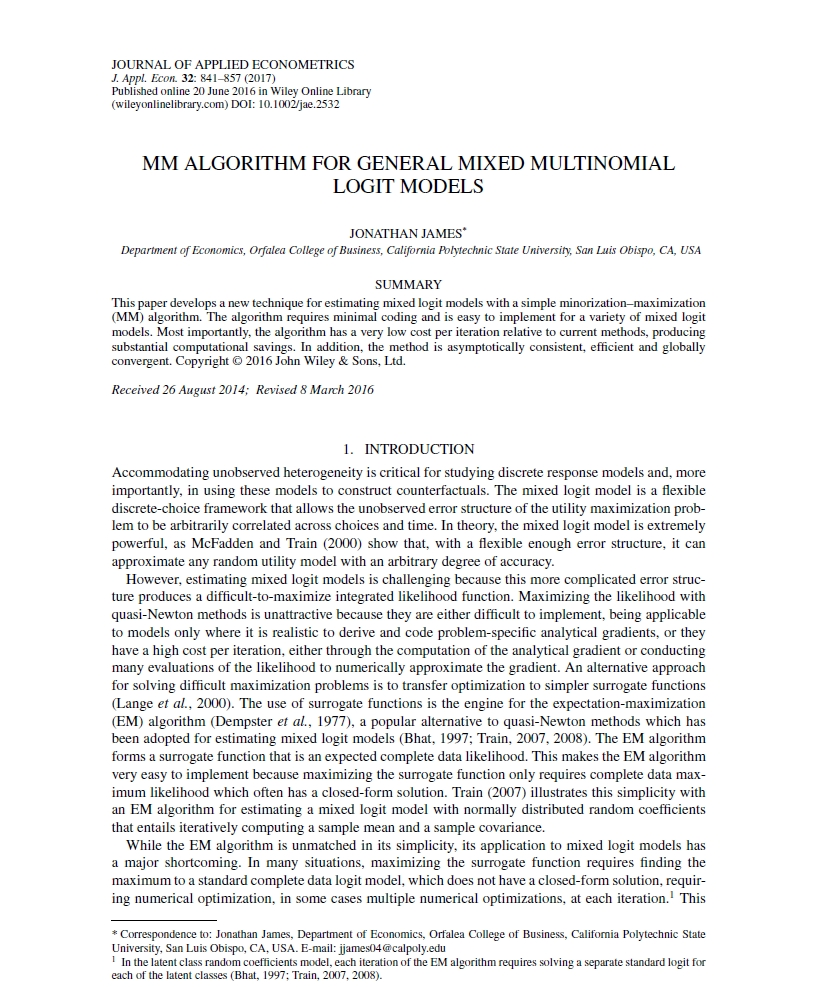
\includegraphics[width=0.5\textwidth]{james_cover.jpg}
\end{frame}




\begin{frame}
\onslide<1->{
Problem: Multinomial logit Hessian depends on $P$'s that change every iteration

\begin{align*}
    H = \sum_i \sum_j P_{ij} x_{ij}x_{ij}'
\end{align*}
}

\onslide<2->{
MM Insight: Replace probability weights with constants to get something like OLS
}

\bigskip{}

\onslide<3->{
Bound Matrix: $B = -\frac{1}{2}\sum_i \left[\sum_j x_{ij}x_{ij}' - \frac{1}{J}\left(\sum_j x_{ij}\right)\left(\sum_j x_{ij}\right)'\right]$
\bigskip{}

No probabilities! Just data $(x_{ij})$ like $X'X$ in OLS
}

\bigskip{}

\onslide<4->{
Result: Compute $B^{-1}$ \textcolor{navy}{once} instead of inverting $P$-dependent matrices every iteration

\bigskip{}

This is why MM is fast
}

\end{frame}




\begin{frame}

\begin{columns}

\begin{column}{0.5\textwidth}
\centering
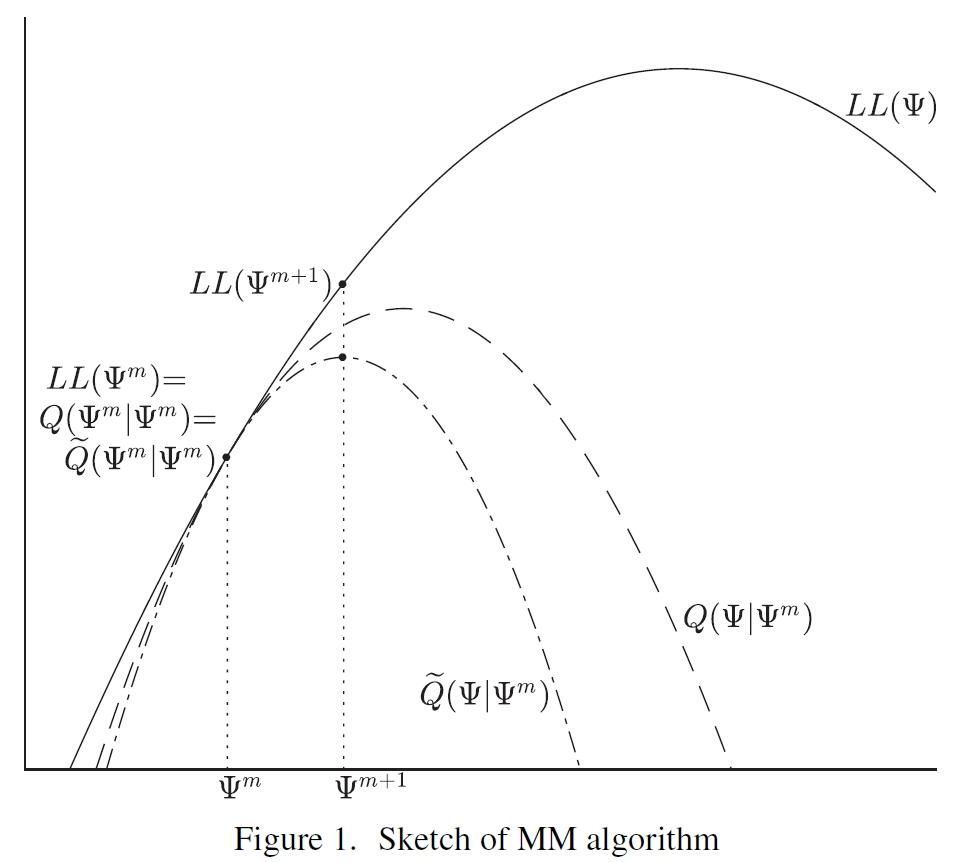
\includegraphics[width=\textwidth]{jamesFig1.jpg}
\end{column}

\begin{column}{0.5\textwidth}

\onslide<2->{
\textbf{$LL(\Psi)$:} Original log-likelihood
\begin{itemize}
\item Complicated, hard to maximize
\end{itemize}

\bigskip{}
}

\onslide<3->{
\textbf{$Q(\Psi|\Psi^m)$:} EM surrogate
\begin{itemize}
\item Bounds $LL$ from below
\item Still requires numerical optimization
\end{itemize}

\bigskip{}
}

\onslide<4->{
\textbf{$\tilde{Q}(\Psi|\Psi^m)$:} MM surrogate
\begin{itemize}
\item Bounds EM surrogate from below
\item Has closed-form solution
\end{itemize}

\bigskip{}

All functions equal at $\Psi^m$, guaranteeing ascent to $\Psi^{m+1}$
}

\end{column}

\end{columns}

\end{frame}



\begin{frame}

MM Algorithm Advantages:

\bigskip{}

\onslide<1->{
\textcolor{navy}{Computational Speed}: 5-8x faster than EM in experiments
}

\bigskip{}

\onslide<2->{
\textcolor{navy}{Memory Efficiency}: Uses sufficient statistics, no need to store simulated datasets
}

\bigskip{}

\onslide<3->{
\textcolor{navy}{Parallelizable}: Unlike EM, easily distributes computations
}

\bigskip{}

\onslide<4->{
\textcolor{navy}{Simple Implementation}: Much easier to code than analytical gradients
}

\bigskip{}

\onslide<5->{
Competitive with quasi-Newton methods, especially for panel data
}

\end{frame}

\begin{frame}

\onslide<1->{
Most beneficial for:
\bigskip{}

\begin{itemize}
\item Models with many fixed coefficients
\item[]
\item Panel data settings
\item[]
\item Complicated models where analytical gradients are impractical
\end{itemize}
}

\bigskip{}

\onslide<2->{
Limitations:
\bigskip{}

\begin{itemize}
\item May require more iterations than EM (especially large choice sets)
\item[]
\item Still requires numerical simulation
\item[]
\item Performance advantage diminishes in cross-sectional data
\end{itemize}
}

\end{frame}

\end{document}